\section{Experimental Results}

\paragraph{Setup.} To evaluate the local planner I ran a batch of seeded random $20\times20$
maps at 30\% obstacle density, restricted to non-trivial start--goal pairs (global path
$\ge 8$ waypoints), each with a 600-step budget.

\paragraph{Comparison against a DWA baseline.} Before settling on MPPI I also implemented the
classic \textbf{Dynamic Window Approach} and ran it through the
identical pipeline as a baseline. DWA evaluates only a single constant command held
over the horizon, so every candidate motion is a circular arc, and from a standstill its
acceleration-limited search window admits only near-zero speeds. Table~\ref{tab:bench} reports
both planners on the same maps.

\begin{table}[h]
    \centering
    \begin{tabular}{lcc}
        \toprule
        \textbf{Local planner} & \textbf{Reached goal} & \textbf{Avg.\ steps (successful)} \\
        \midrule
        MPPI (chosen method) & \textbf{17 / 25 (68\%)} & 208 \\
        DWA (baseline) & 0 / 25 (0\%) & --- \\
        \bottomrule
    \end{tabular}
    \caption{Goal-reaching success over 25 non-trivial maps. Both planners use the same
    aligned A* path and probabilistic cost; only the optimiser differs.}
    \label{tab:bench}
\end{table}

MPPI reached the goal on 68\% of maps while DWA, under the identical pipeline, reached none
--- it stalls in the local-minima traps analysed in Section~8, which is exactly why I chose
MPPI as the primary method. Figure~\ref{fig:result} shows a representative MPPI run: the
executed trajectory (red) tracks the A* path (dashed blue) through the clutter while staying
in the low-risk (green) band of the field, rounding corners smoothly rather than cutting them.

\begin{figure}[h]
    \centering
    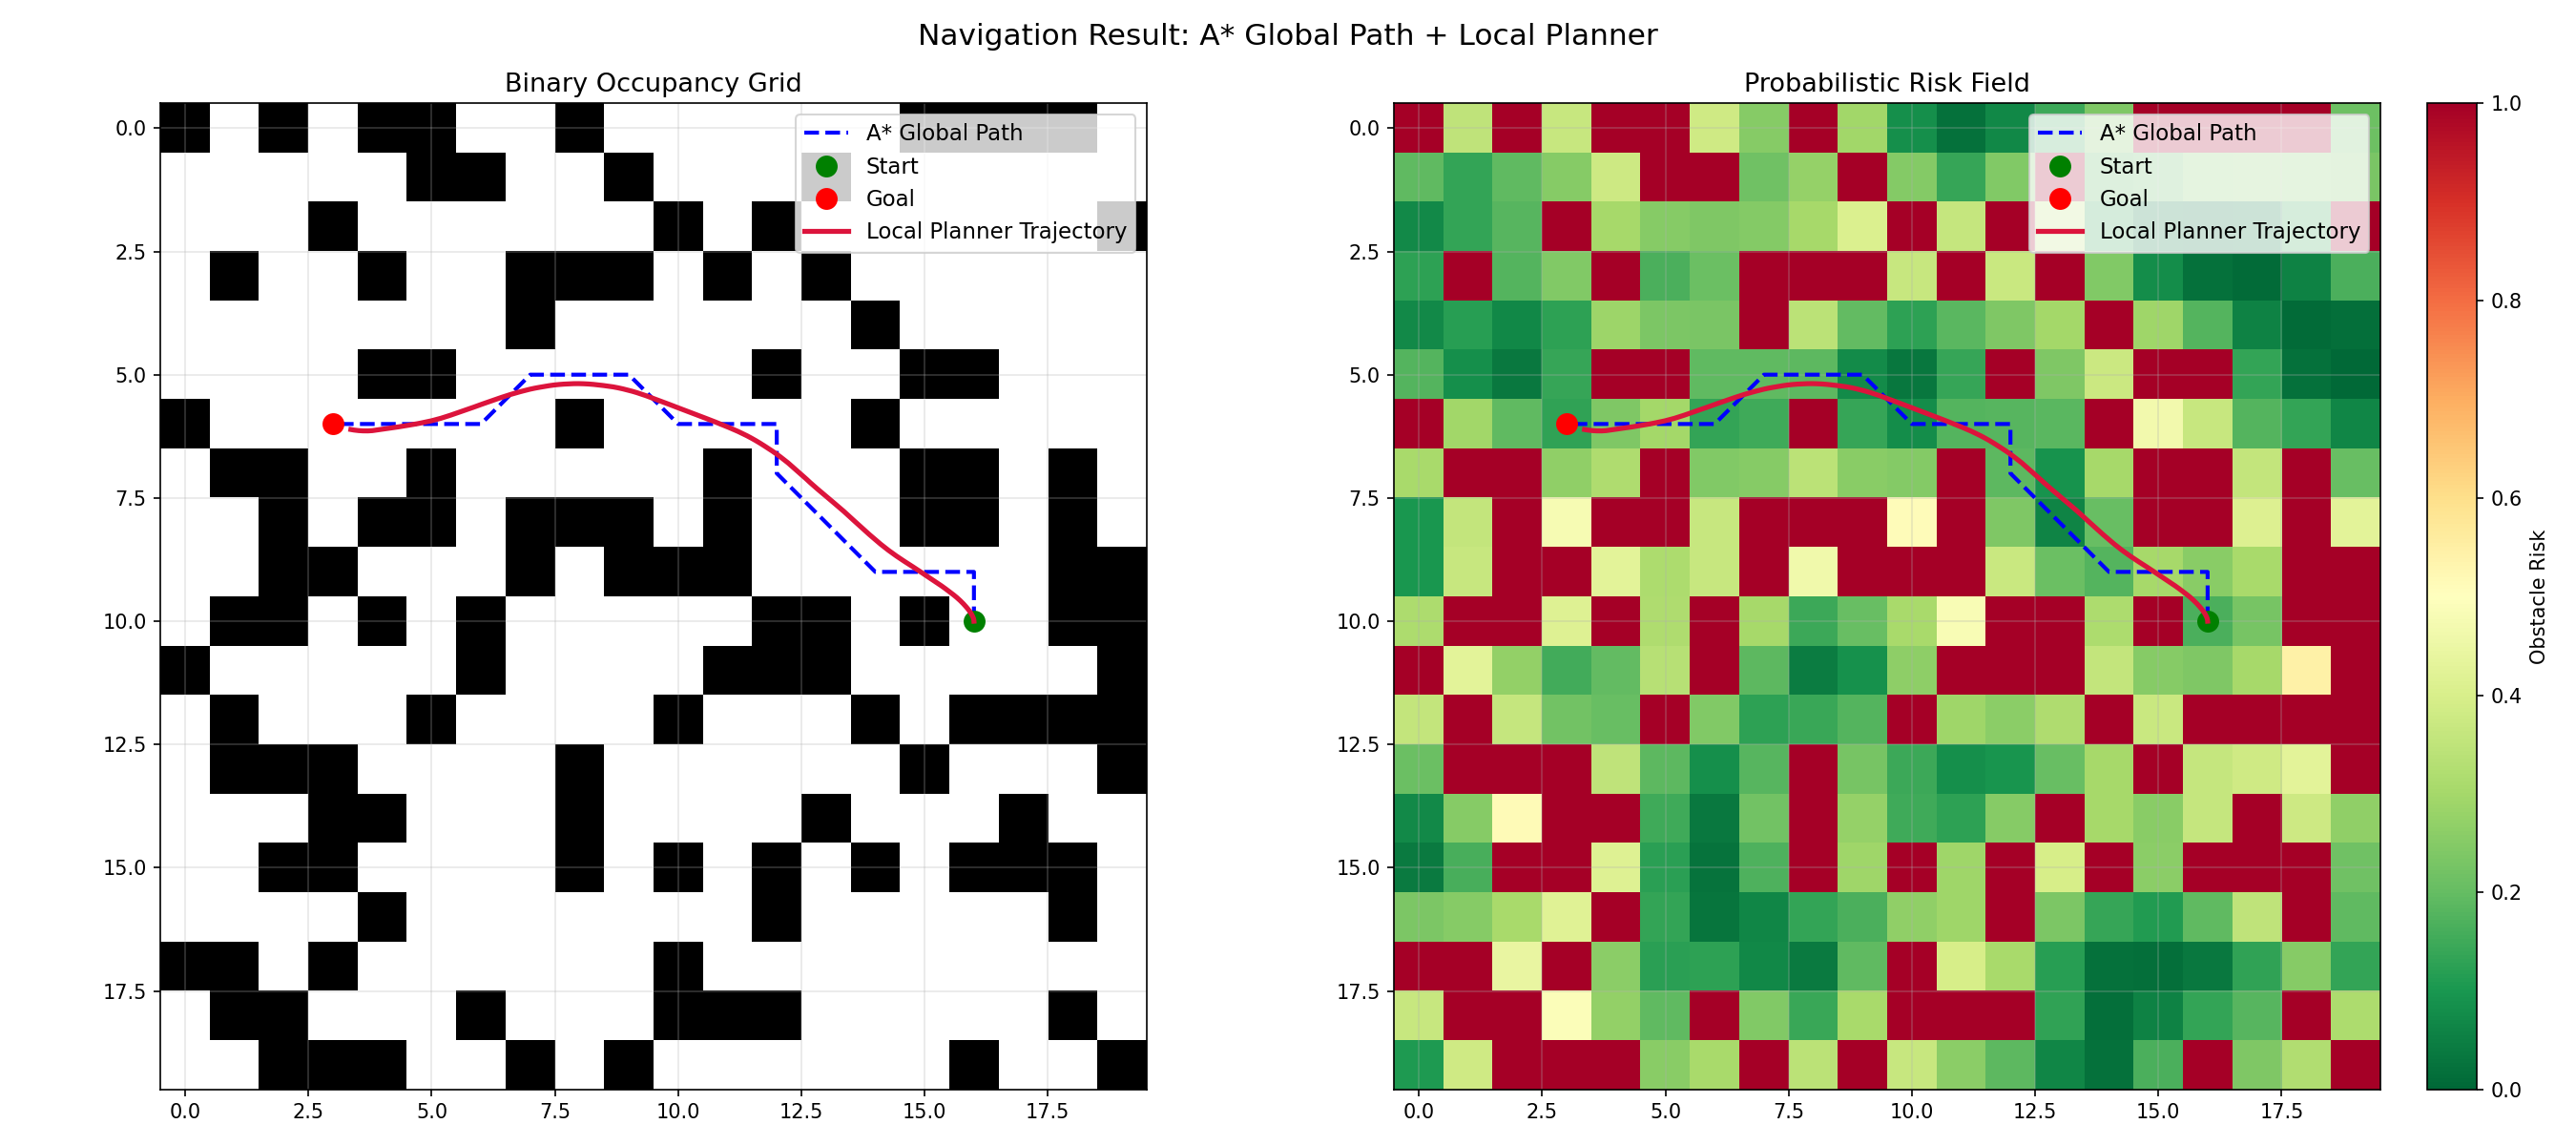
\includegraphics[width=0.82\textwidth]{../experiments/dwa_result.png}
    \caption{Navigation on a $20\times20$ map (30\% density). Left: binary grid. Right:
    probabilistic risk field (red = high, green = safe). Dashed blue: A* global path.
    Solid red: executed MPPI trajectory.}
    \label{fig:result}
\end{figure}

I also observed the effect of weighting: raising the obstacle weight widens the
robot's clearance but slows it and can freeze it in tight passages, while raising the
velocity/goal weights speeds it up at the cost of closer, riskier passes --- a concrete
speed/safety trade-off.
